\documentclass{article}

\usepackage{graphicx}
\usepackage{xr}
\graphicspath{{../figures/}}

\begin{document}

\title{Supplementary Materials \\
    Diagnostic performance of quantitative measures from FDG-PET/CT, FEC-PET/CT and DW-MRI in the detection of lymph node metastases in endometrial and cervical cancer.}

\author{Ben King \\ b.g.king@sms.ed.ac.uk}

\maketitle

\begin{table}[h]
    \centering
    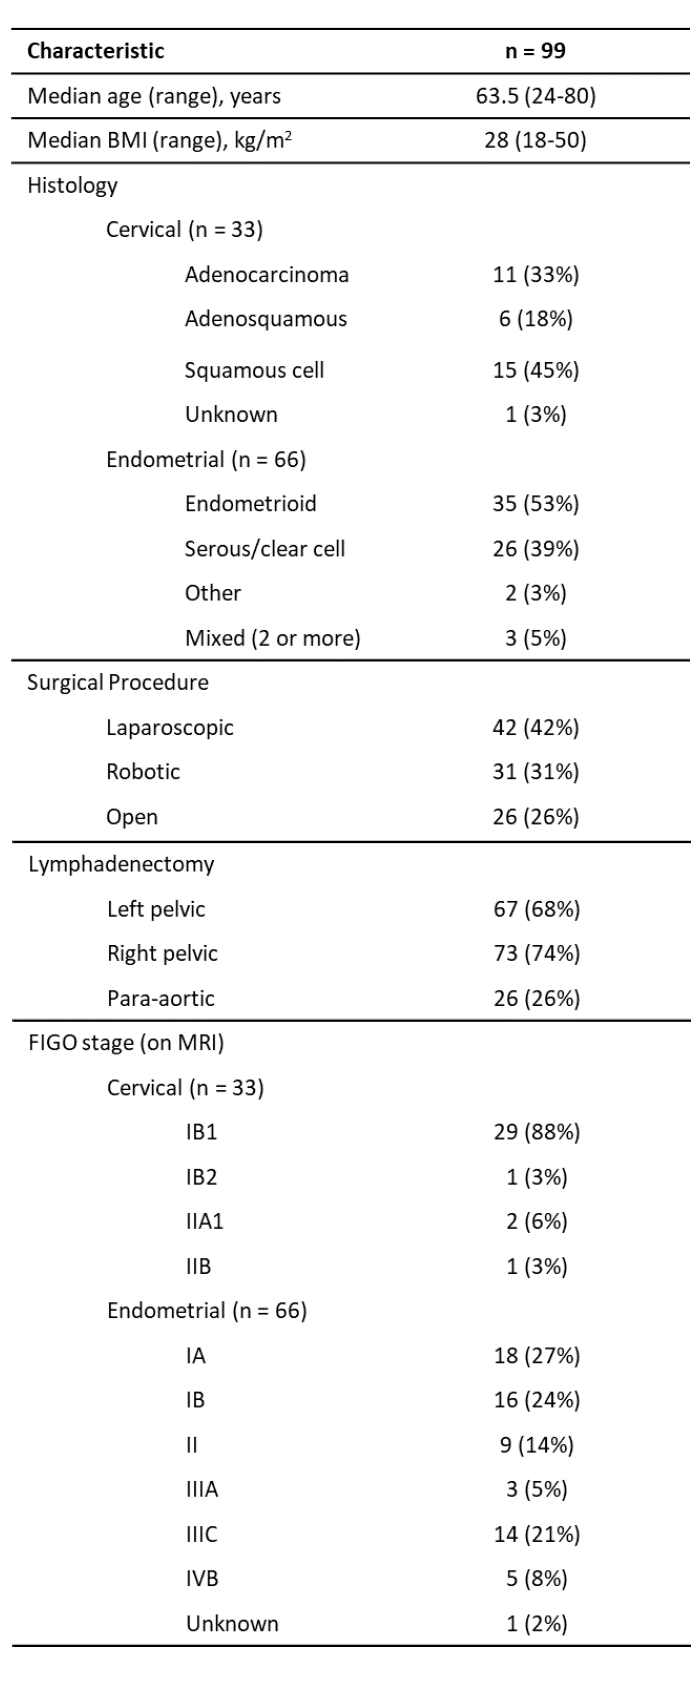
\includegraphics[width=0.5\textwidth]{tables/demographics}
    \caption{Demographics of patients enrolled onto the MAPPING study and eligible for analysis by meeting the primary reference standard of surgically confirmed nodal histology.}
    \label{table:demographics}
\end{table}

\begin{figure}[h]
    \centering
    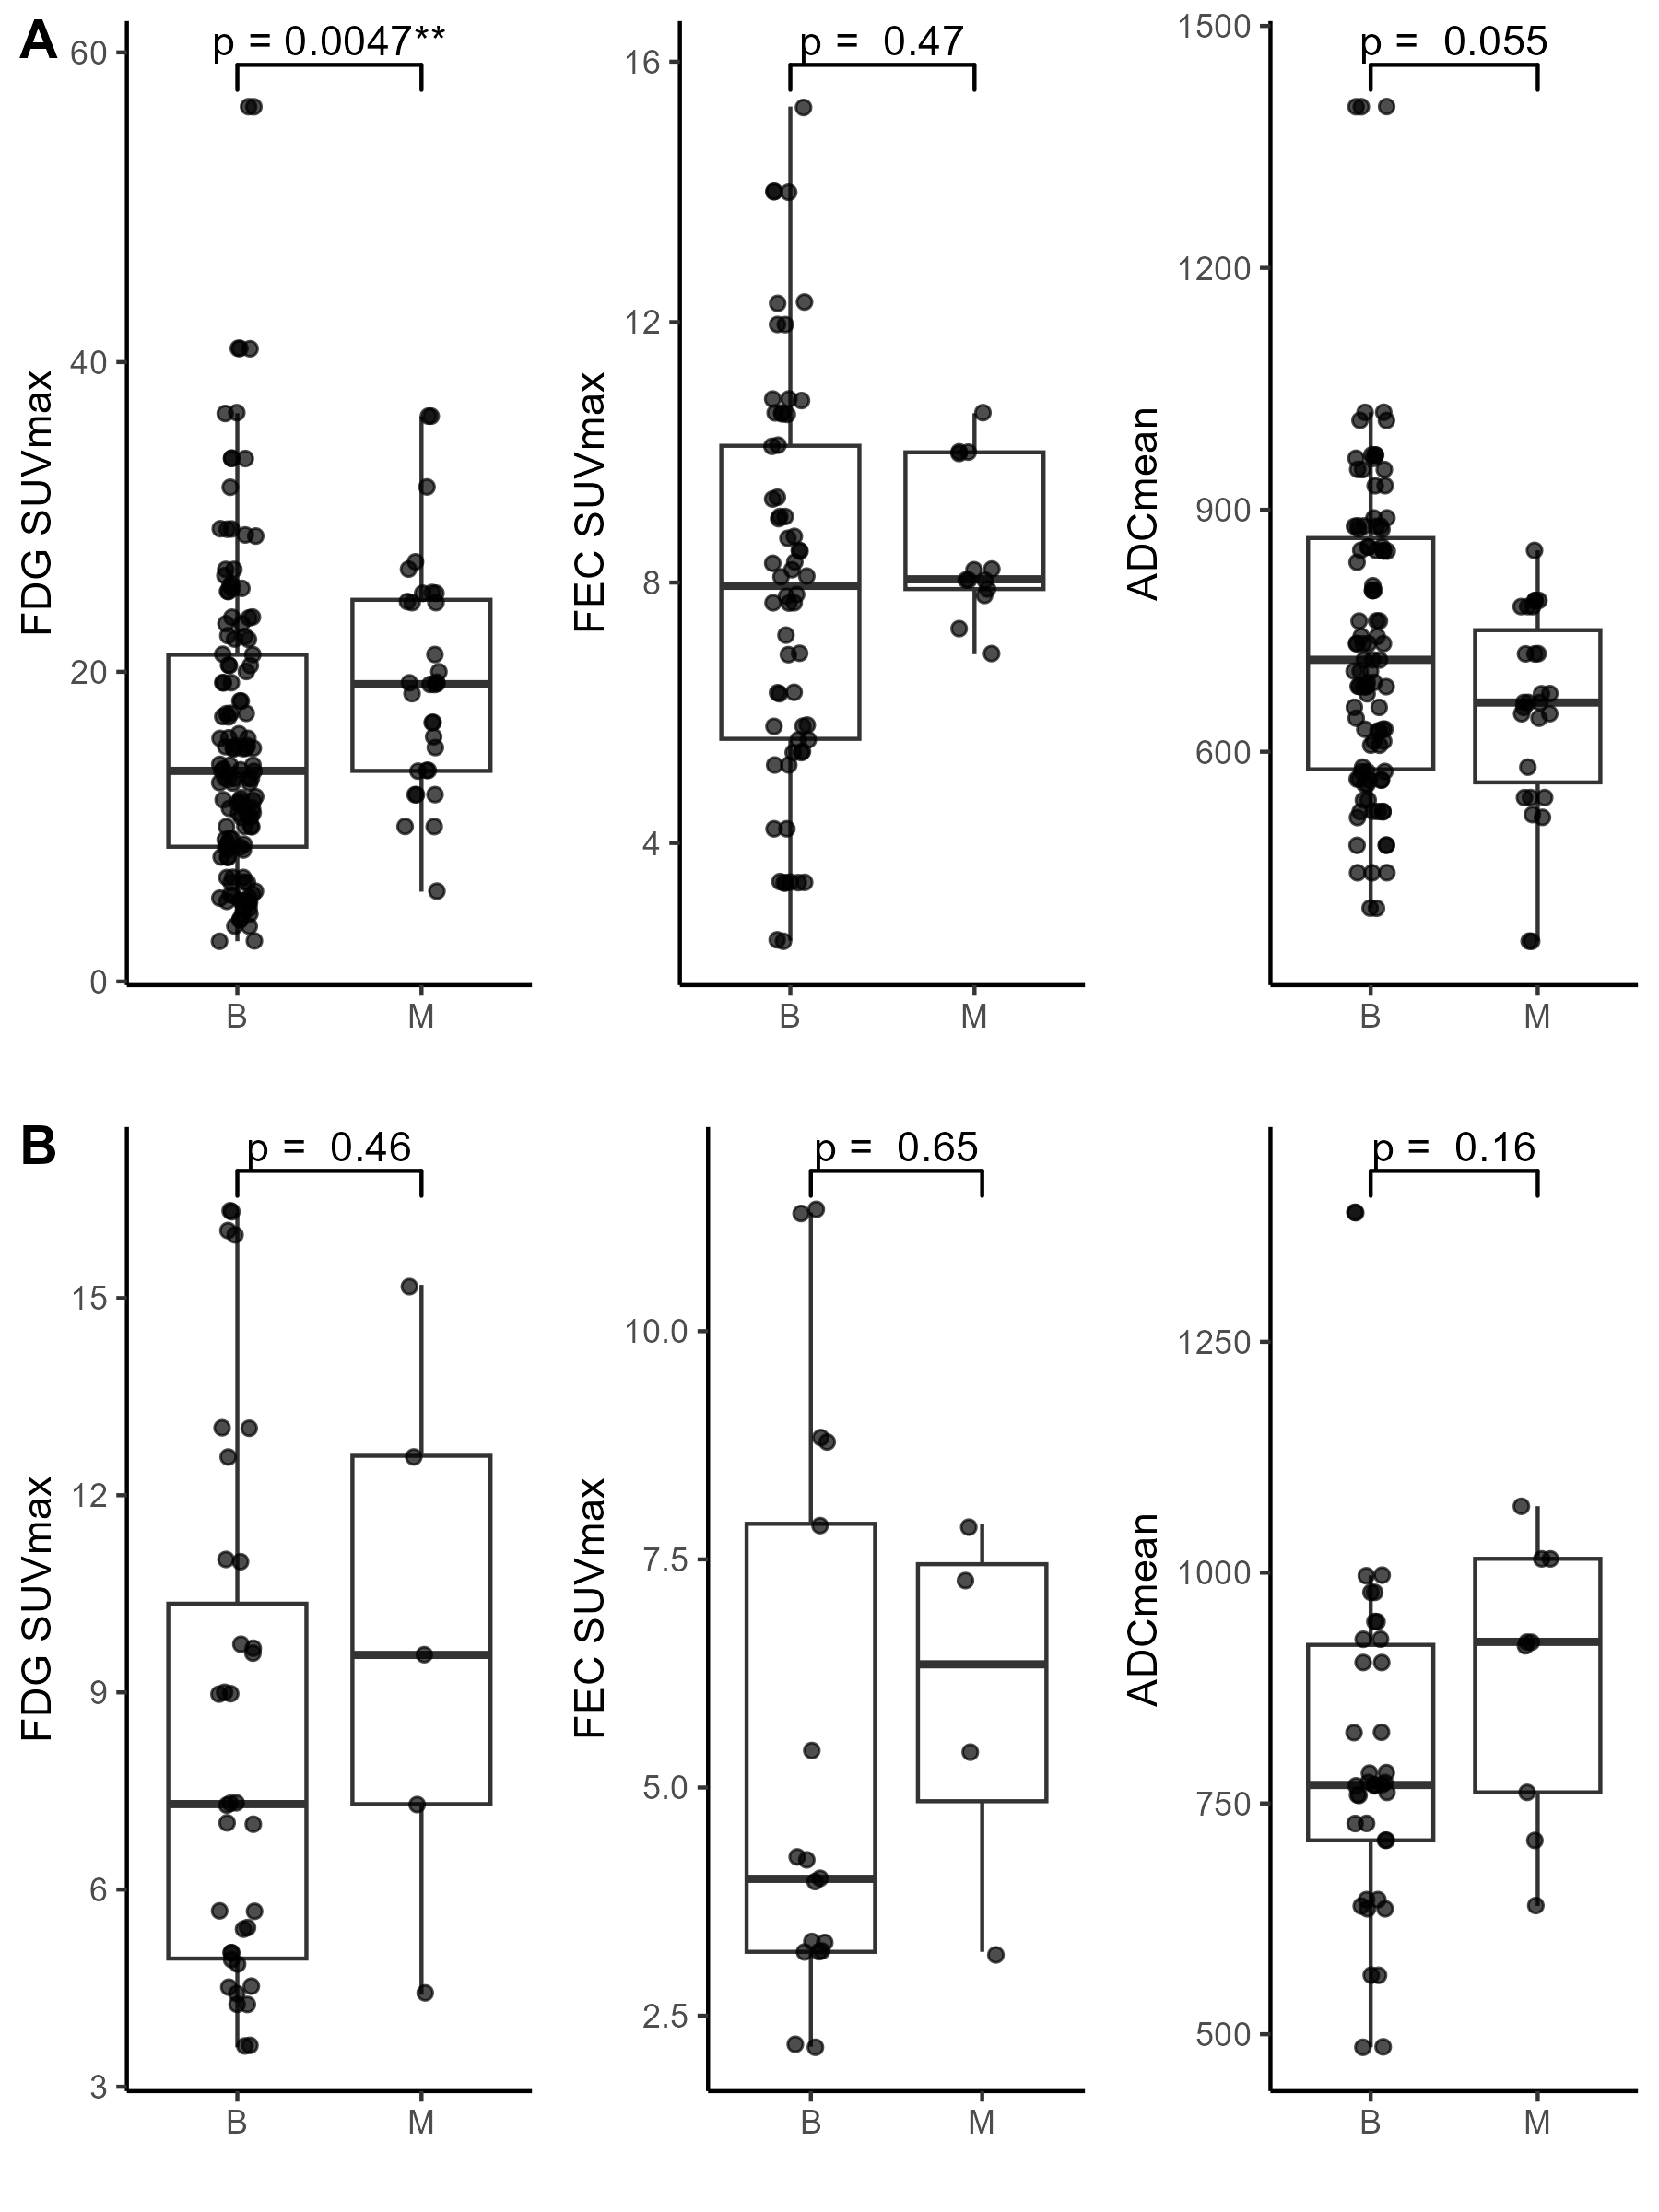
\includegraphics[width=0.75\textwidth]{quants_pt_byCancer}
    \caption{
        (A) SUVmax was significantly elevated in primary tumours on FDG-PET/CT in patients with malignant (M) lymph nodes compared to those with benign (B) lymph nodes in endometrial cancer. (B) No significant difference in quantitative measures of the primary tumour were found for any imaging modality in cervical cancer. **, p $<$ 0.01.
         }
    \label{fig:quants_pt_byCanc}
\end{figure}

\end{document}